\documentclass[10pt,twocolumn,letterpaper]{article}

\usepackage{cvpr}
\usepackage{times}
\usepackage{epsfig}
\usepackage{graphicx}
\usepackage{amsmath}
\usepackage{amssymb}

\usepackage{caption}
\usepackage{subcaption}

% Include other packages here, before hyperref.

% If you comment hyperref and then uncomment it, you should delete
% egpaper.aux before re-running latex.  (Or just hit 'q' on the first latex
% run, let it finish, and you should be clear).
%\usepackage[pagebackref=true,breaklinks=true,letterpaper=true,colorlinks,bookmarks=false]{hyperref}

\cvprfinalcopy % *** Uncomment this line for the final submission

%\def\cvprPaperID{****} % *** Enter the CVPR Paper ID here
%\def\httilde{\mbox{\tt\raisebox{-.5ex}{\symbol{126}}}}

% Pages are numbered in submission mode, and unnumbered in camera-ready
\ifcvprfinal\pagestyle{empty}\fi
\begin{document}

%%%%%%%%% TITLE
\title{Breadboard to Schematic}

\author{Catherine Olsson \\
MIT\\
{\tt\small catherio@mit.edu}
% For a paper whose authors are all at the same institution,
% omit the following lines up until the closing ``}''.
% Additional authors and addresses can be added with ``\and'',
% just like the second author.
% To save space, use either the email address or home page, not both
\and
Michele Pratusevich\\
MIT\\
{\tt\small mprat@mit.edu}
}

\maketitle
\thispagestyle{empty}

%%%%%%%%% ABSTRACT
\begin{abstract}

TODO: Write the abstract.

\end{abstract}

%%%%%%%%% BODY TEXT
\section{Introduction}

Breadboards are an important tool for do-it-yourself hardware
designers to quickly test circuit systems. They are easy to assemble,
easy to change, and easy to test, so are the tool of choice for the
first prototype of many hobbyists and students. A
programmatically-drawn, or more likely hand-drawn, schematic diagram
is used to prototype the circuit board, but if the circuit is going to
be used for high-speed, low-noise, or multiple-production
applications, a printed circuit board (PCB) is much more desirable
than a breadboard. However, it can be time-consuming to enter a
breadboard's connection map into a programmatic language that can be
used to generate a PCB. It would be faster to create a PCB-ready
representation directly from the circuitboard. Even if the result had
errors, these could be corrected by the user in less time than it
would take to create the representation from scratch.

Our approach to solve this problem was a vision-based tool to
go from a picture of a breadboard circuit to a file written in a
PCB-ready format given by Eagle. Although a fully-automated tool
proved to be too large a task for this project, we have successfully
implemented a GUI-based tool that spans the full pipeline from
bitmap image input to PCB-ready output by incorporating automated
methods with input from the user.

Overall, this project was an exercise not only in computer vision
methods for recognition and segmentation, but also in more general
problems of visualization; modularity; and designing, manipulating,
and transforming between representations on a spectrum from
concrete (pixel-level) to abstract (component-level).

%-------------------------------------------------------------------------

\section{Related Work}

TODO, if any

%-------------------------------------------------------------------------

\section{Background}

\subsection{Properties of Breadboards}

When solving vision-based problems, it is critical to know your system
properties to better develop algorithms customized to the strengths and
weaknesses of a particular application. Photos of breadboards have a number of
interesting properties that can be useful in segmentation, identification, and
restructuring tasks. A number of visually-interesting properties are listed here:
\begin{itemize}
\item A single component on a breadboard, such as a wire, LED, or chip is often a single color. 
\item The colors of the various components are often easily visually distinguishable. 
\item The breadboard is often square with the image. 
\item The breadboard, when not covered with components, has a black checkered pattern of holes in it. 
\item The breadboard color is relatively constant over the entire breadboard, except for the holes.
\item Breadboards follow a specific connectivity pattern. In Figure \ref{fig:board}, each column (not including the top two and bottom two rows) can be considered a single connection. The middle gap in the square holes is a break in the connection for each column, so there are five total holes connected to one connection in each of the columns. The top two and bottom rwo rows are connected horizontally into a single connection. Typically, one denotes a voltage of $+5$ volts and one denotes \verb|GND|, or $0$ volts. 
\end{itemize}

\begin{figure}[t]
\begin{center}
   %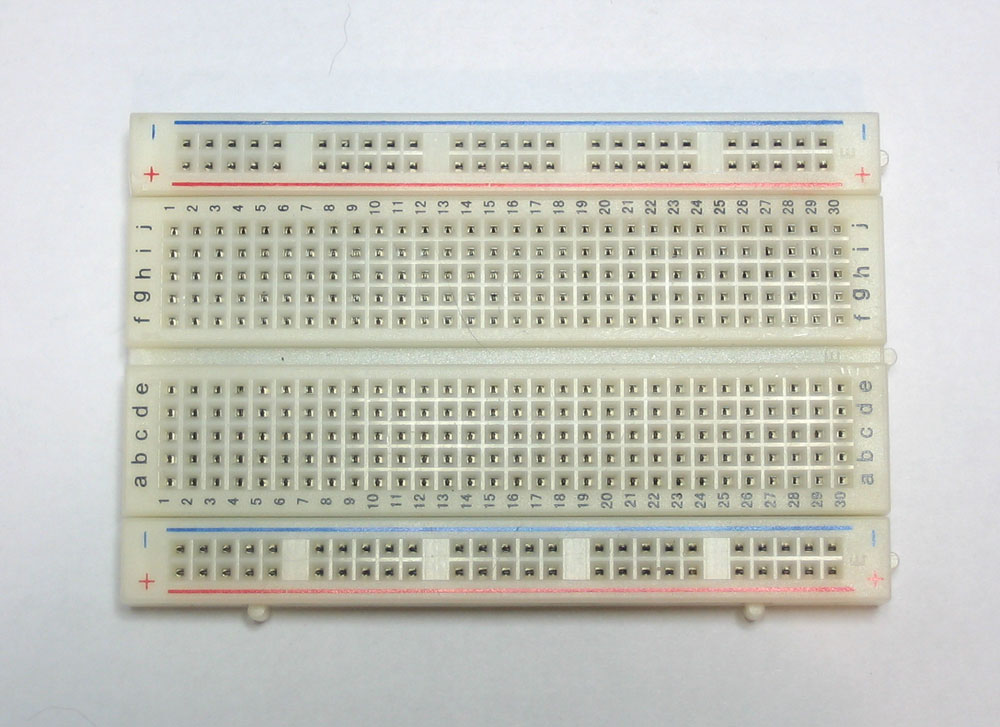
\includegraphics[width=0.8\linewidth]{imgs/breadboard.jpg}
\end{center}
   \caption{A breadboard oriented like those oriented in images that
     we can process, before any components have been added to it}
\label{fig:board}
\end{figure}

\subsection{Schematic-drawing Software}

The Eagle program, developed by CADSoft, is a free schematic and PCB-drawing
software that translates schematics into a PCB-ready format. The Eagle file
format is a type of XML, which makes it easy to programmatically update from an
image. Eagle PCB and schematic diagrams are based off of the same language, so
drawing a schematic in Eagle is sufficient to computing the full PCB. 

%-------------------------------------------------------------------------

\section{User Interface of our Tool}

From the point of view of the user, the workflow of our tool is as
follows:

\begin{enumerate}
\item Start the program, indicating the filename of the bitmap image
  containing a photograph of the breadboard.
\item Select the most important colors in the image. For example, a
  beige breadboard with red and green wires and a black microchip
  would require the user to click on examples of those four colors.
\item Confirm the selected colors to view a segmentation map of the image
  based on those colors.
\item Select the components in the segmentation map which should be
  analyzed and included in the final schematic.
\item Confirm the selected components and obtain an XML version of
  their connectivity.
\end{enumerate}

In the following sections we will explain more about our approach to
the problem, the results we obtained, and the limitations of our tool
and techniques.

%-------------------------------------------------------------------------
\section{The Approach}

The problem of translating information from a picture of a circuit to a
PCB-friendly file format has two main steps. First, the components must be
identified in the image, and second, the components must be placed in a virtual
grid representation independent of their relation in the image. 

For our implementation we chose to use python and it's Tkinter, PIL, SciPy, and
Numpy packages for ease of implementation, user interface, and speed. 

%-------------------------------------------------------------------------
\subsection{Segmentation into Circuit Components}

At first we were unsure about which approach towards segmentation into image
components was going to be more effective, so we tried two algorithms for
detecting components. 

\subsubsection{Color Following}

As a first step to tackling the component segmentation problem, we took
advantage of the natural segmentation in a breadboard picture according to
color. Components on a breadboard are different colors that are localized in
one location, so to take advantage of this, we developed an algorithm that
``grows'' a component based on a given color pixel. A seed color is given to
the algorithm and added to an active set of pixels. For each neighbor of each
pixel in the active set, the decision is made whether that pixel is in the
component if the pixel does not change the running RGB color-average of all the
pixels current in the component. If a pixel is added to a component, it is then
also added to the active set and the algorithm continues.     

The main problem with this algorithm is that it is highly dependent on the seed
pixel to the image. If a pixel is chosen that is too dark for example, the
running average that the algorithm will calculate will be off from the actual
running average of the color of the component, so the algorithm will return
incorrect results.   

\subsubsection{Segmentation by Nearest Color}

Idea is to segment on color by quantizing the color of the
image and finding connected components in the quantized color space.

Overall algorithm:
\begin{enumerate}
\item Use a 3D clustering algorithm to find representative colors. We
  wanted to use k-means, but it didn't work. The user picks these.
\item Map colors to the nearest representative color- ie, divide up
  the colorspace into Voronoi regions with Euclidean distance in
  RGB-space.
\item Find connected components of each color. Standard algorithms
  work on binary masks, so run each color independently
\item (Optional) Eliminate small connected components using binary
  erosion/propagation. We got this part working, but it is not needed
  in the current user-assisted workflow.
\end{enumerate}

Shows some problems, but generally works well enough for this application.

\subsection{Occlusion Handling}

A problem with breadboard circuits is often that components (most often wires)
are occluded from each other. This is a critical issue that in any finalized
version of a product like this needs to be addressed. Because we ran into other
issues with our approach, we were not able to effectively solve the occlusion
problem.  

\subsection{Virtual Grid Representation}

The next component of the project involved translating the component data into
a schematic. Knowing all the pixel locations that make up a component, we
calculate the end pixel positions of each component rounded to the nearest
$10$. Because components are aligned to the hole-grid that is present on the
breadboard, the calculated endpoints of the components can be used to place
components on a grid in the schematic. The rounded values for the $x$ and $y$
coordinates are used to place the components into their XML representations
into the schematic. 

After all components are identified and represented in their XML formats, a new
file is constructed with the proper sschematic-XML information.    

%-------------------------------------------------------------------------
\section{Results}

\subsection{The Full Spectrum}

Running our system using the nearest-color algorithm for segmentation yielded
very positive results. Figure \ref{fig:origfull} shows the original image
operated under, and Figure \ref{fig:segfull} shows the image after
segmentation. The final schematic result (opened as a file in Eagle) is shown
in Figure \ref{fig:schemfull}. 

Notice how the schematic figure is upside down of the original image and it's
segmentation; this is a result of the difference in indexing conventions
between PIL, numpy, and Eagle.

\begin{figure}[ht]
\centering
\begin{subfigure}[b]{\linewidth}
	\centering
   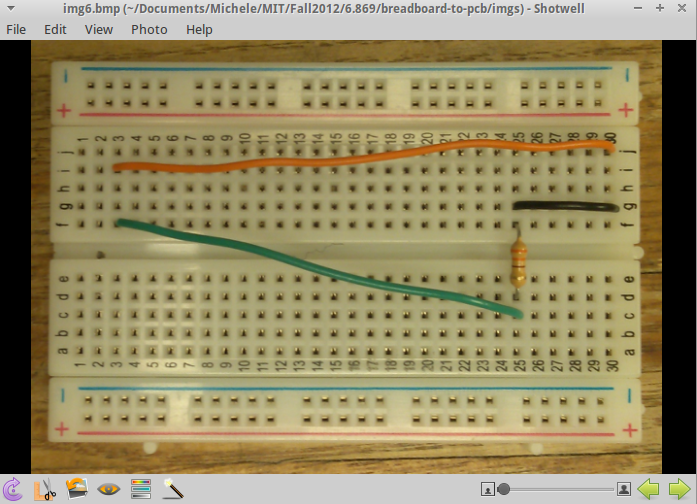
\includegraphics[width=0.9\linewidth]{demos/full_pipeline2_original.png}
	\caption{The original image}
	\label{fig:origfull}
\end{subfigure}
\begin{subfigure}[b]{\linewidth}
	\centering
   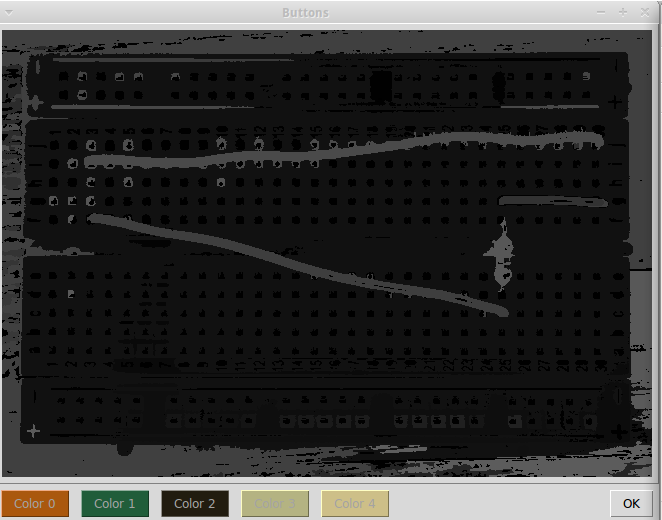
\includegraphics[width=0.9\linewidth]{demos/full_pipeline2_segmentation.png}
	\caption{The original image after the segmentation into components}
	\label{fig:segfull}
\end{subfigure}
\begin{subfigure}[b]{\linewidth}
	\centering
   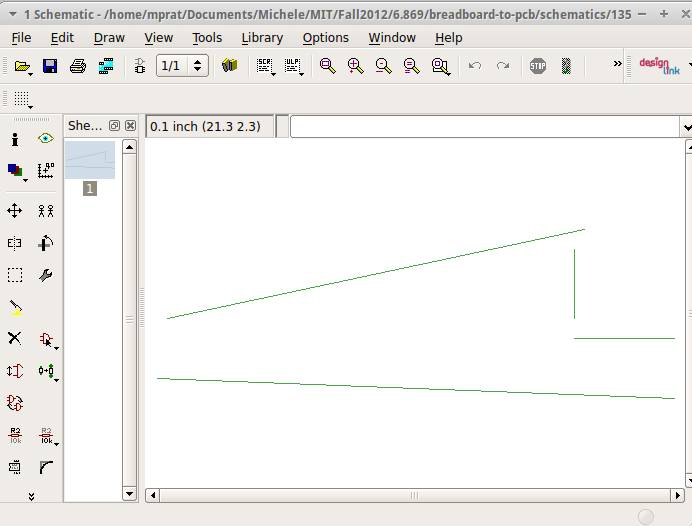
\includegraphics[width=0.9\linewidth]{demos/full_pipeline2_schematic.png}
	\caption{The schematic computed from the original image}
	\label{fig:schemfull}
\end{subfigure}
\end{figure}

\subsection{Comparing Color-following and Segmentation by Nearest Color}

The color-following and nearest-color algorithms solve somewhat different
problems. The color-following algorithm assumes a seed pixel (whether given
programmatically or by a user) and constructs a component from that seed pixel,
while the nearest-color algorithm separates the image into sections based on
colors found in the entire image. In both bases, if the same component is
found, it should be found correctly. Given that the exact parameters for both
algorithms were not perfectly tuned, these results are a comparison of the
current implementations of the algorithms as we have them.

\begin{figure}[ht]
\centering
\begin{subfigure}[b]{\linewidth}
	\centering
   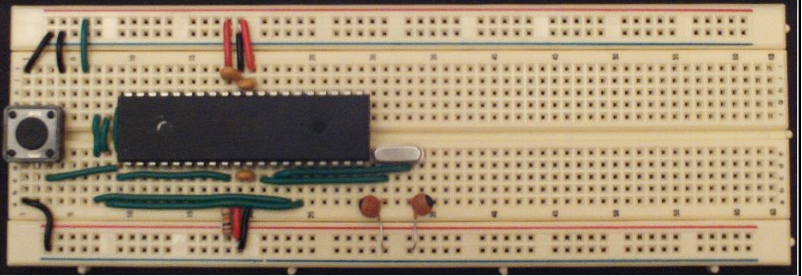
\includegraphics[width=0.9\linewidth]{demos/original_of_comp.png}
	\caption{The original image}
	\label{fig:origcomp}
\end{subfigure}
\begin{subfigure}[b]{\linewidth}
	\centering
   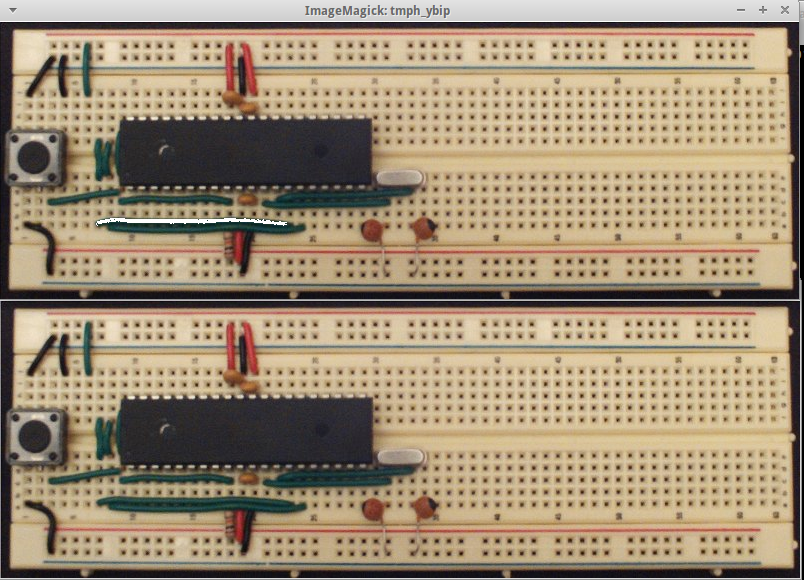
\includegraphics[width=0.9\linewidth]{demos/single_wire_not_double.png}
	\caption{The white wire detected by the color-following algorithm}
	\label{fig:cfollow}
\end{subfigure}
\begin{subfigure}[b]{\linewidth}
	\centering
   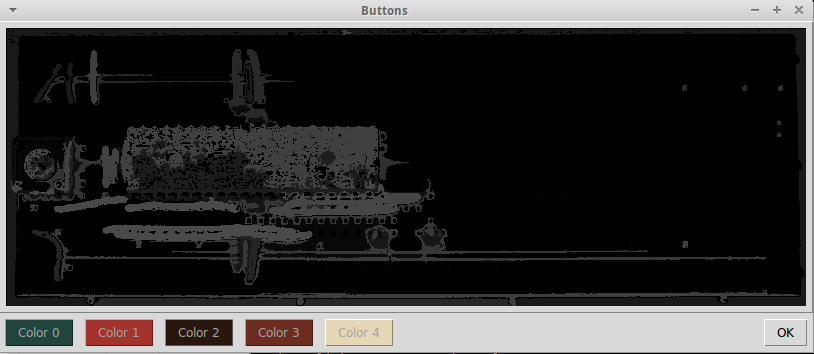
\includegraphics[width=0.9\linewidth]{demos/closest_color.png}
   \caption{Note the same wire incorrectly detected by the closet-color algorithm}
	\label{fig:ncolor}
\end{subfigure}
\end{figure}

Figure \ref{fig:origcomp} has the original image that we are analyzing. Figure
\ref{fig:cfollow} shows one wire detected by the color-following algorithm.
Note how, given a particularly good seed color, it was able to only detect one
of the two wires that are nearest each other. In Figure \ref{fig:ncolor}, note
the same wire is detected as a single wire with the wire immediately below it. 

\subsection{Limitations}

One limitation of our product as we've written it is that it can only handle
breadboard circuits that are oriented horizontally as shown above in Figure
\ref{fig:board}. This is because connectivity properties of the breadboard are
geometry-dependent, and our program automatically assumes a particular
orientation for the breadboard to infer connectivity.  

%-------------------------------------------------------------------------
\section{Future Work}

TODO: automatically identify components

%-------------------------------------------------------------------------
\section{Conclusion}

TODO

{\small
\bibliographystyle{ieee}
\bibliography{egbib}
}

\end{document}
